%
% Diseño de programa tokenizador, capítulo de análisis y diseño.
% Proyecto Lovelace.
%

\subsection{Diseño de programa tokenizador}

En la sección \ref{sec:algoritmos} se enlistaron y detallaron los algoritmos
tokenizadores que implementaremos. En esta sección se describe, mediante
\gls{gl:uml}, la estructura del programa generador de \glspl{gl:token}.

\subsubsection{Vista estática del programa}

En el diagrama de la figura \ref{clases_general} se muestra una vista estática
general del programa. Las clases se dividen en dos paquetes: implementaciones
y utilidades. Las utilidades abarcan estructuras de datos, interfaces,
clases de excepciones y clases de prueba; todas ellas no tienen que ver
de forma directa con criptografía, sino que se trata de código de soporte
para las implementaciones. En las implementaciones van no solamente
los algoritmos presentados en la sección \ref{sec:algoritmos}, sino que todas
las demás clases (generalizaciones, utilidades, implementaciones de
soporte) que están relacionadas con los algoritmos tokenizadores; en el caso
de este paquete, sí todo está relacionado o con criptografía o con un
entorno bancario.

La figura \ref{paquetes_general} muestra la dependencia entre los paquetes que
componene al programa: las implementaciones importan el contenido de las
utilidades; ambos paquetes cuentan con equivalentes de prueba (más adelante se
detalla el funcionamiento de las pruebas), en donde cada uno importa el paquete
que está probando.

Retornando al diagrama \ref{clases_general}: muestra solamente las clases
e interfaces directamente relacionadas con los algoritmos tokenizadores;
en las próximas secciones se mostrarán algunas otras vistas. Las utilidades
contienen las interfaces para definir los distintos tipos de funciones y la
estructura de datos (Arreglo) que se usa de manera constante en todo el
programa. Las implementaciones muestran las interfaces que definen y clasifican
a los algoritmos tokenizadores; también se muestra (por razones de espacio,
solo el nombre) las clases concretas de los sistemas tokenizadores.

Las interfaces de las funciones utilizan plantillas para definir las propias
firmas de los métodos abstractos que declaran. Esta es una forma bastante
efectiva para hacer diseños débilmente acoplados (ver
\gls{gl:acomplamiento}): por ejemplo, las redes Fesitel necesitan
de una función de ronda sobre la que \textit{no necesitan} saber nada en
particular, solo necesitan saber que la clase define un método \textbf{operar},
que es con lo que funciona el algoritmo definido por la red.

El Arreglo es una implementacion propia de una estuctura de datos de
almacenamiento secuencial. Es solamente una interfaz a una sección
de memoria (un arreglo tradicional); sin embargo, lo importante de este es
que imita el formato de las estructuras de la librería estándar de C++
(esquema de constructores y destructores para gestión de memoria, uso
de plantillas para programación genérica, etcétera). El arreglo de dígitos es
una especialización que mantiene una representación interna tanto en cadena como
en número; este arreglo es el que ocupan para comunicarse todos los
algoritmos tokenizadores. Por esta última razón es por la que se
mantienen las dos representaciones internas: algunos métodos requieren
interpretar las entradas como números y otros como cadenas.

Los algoritmos tokenizadores implementan la interfaz definida por las
funciones con inverso definiendo el tipo de ida y de vuelta como un
arreglo de dígitos (\gls{gl:pan} y \gls{gl:token}). Las interfaces intermedias
(algoritmos reversibles e irreversibles) permiten definir un comportamiento
genérico para cada tipo de algoritmo; estas a su vez declaran los métodos
abstractos que los algoritmos concretos deben de implementar.

\begin{figure}
  \begin{center}
    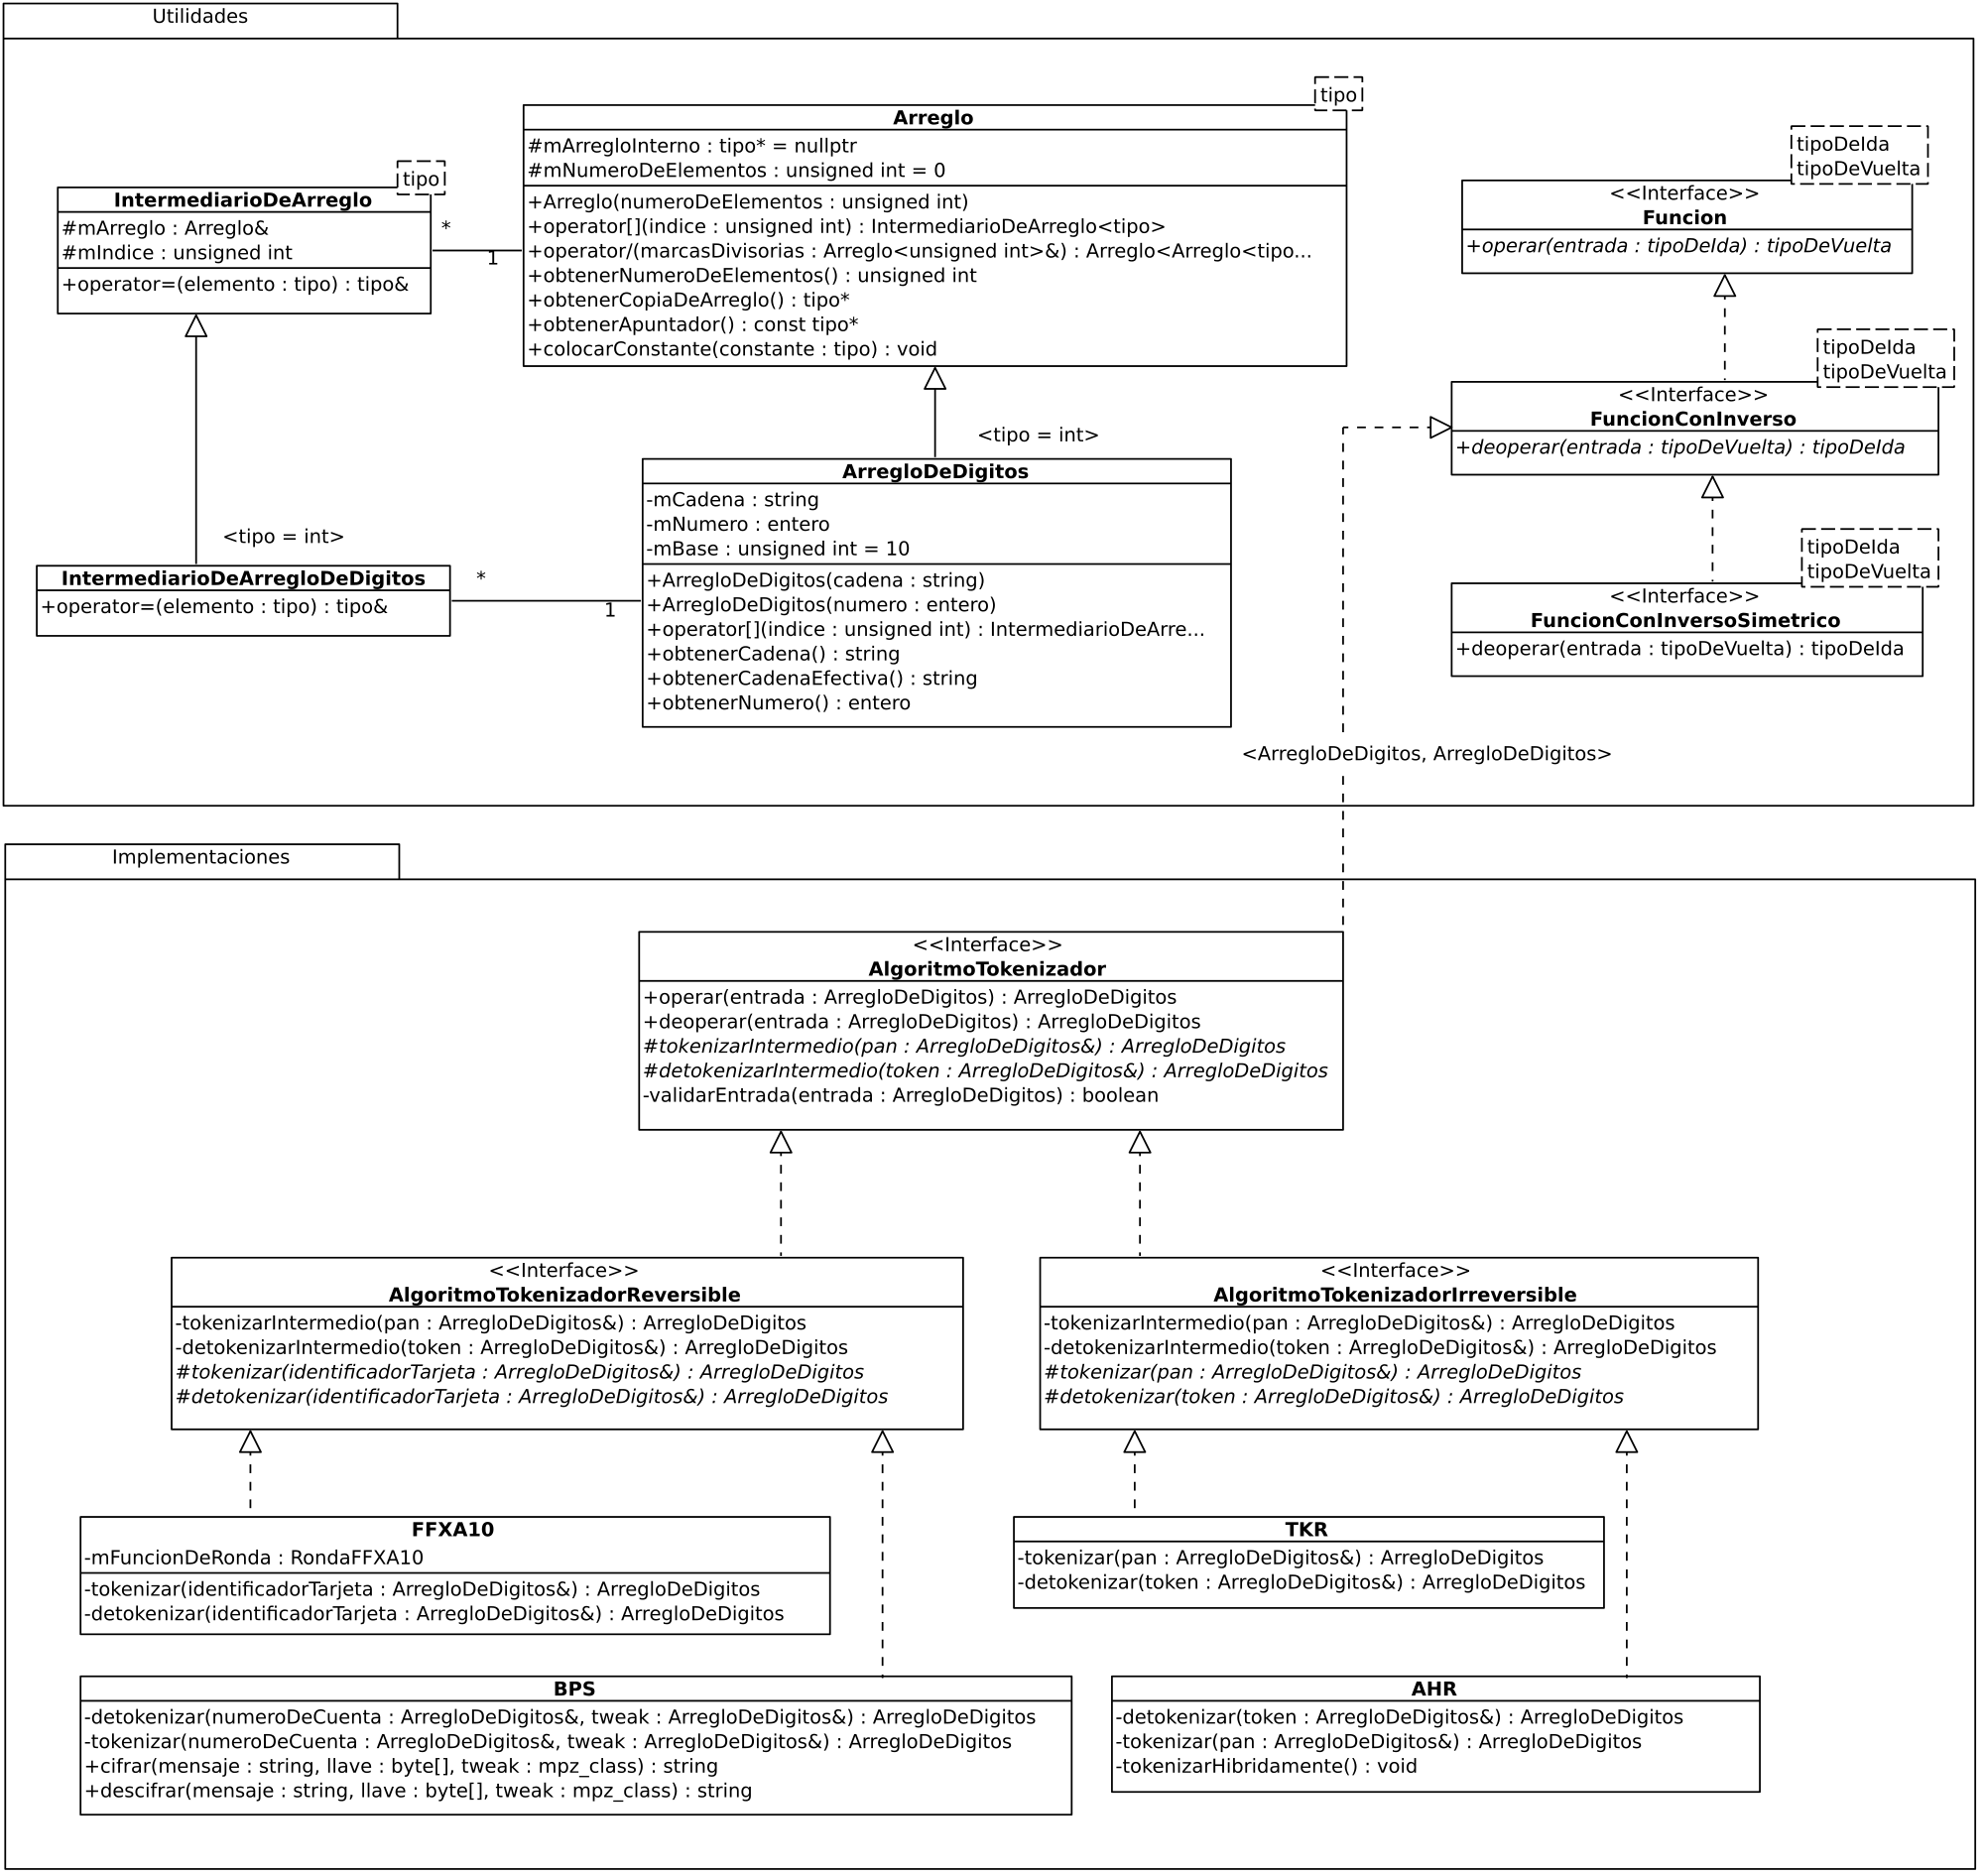
\includegraphics[width=1.0\linewidth]{diagramas/diagrama_general.png}
    \caption{Diagrama de clases general.}
    \label{clases_general}
  \end{center}
\end{figure}

\begin{figure}
  \begin{center}
    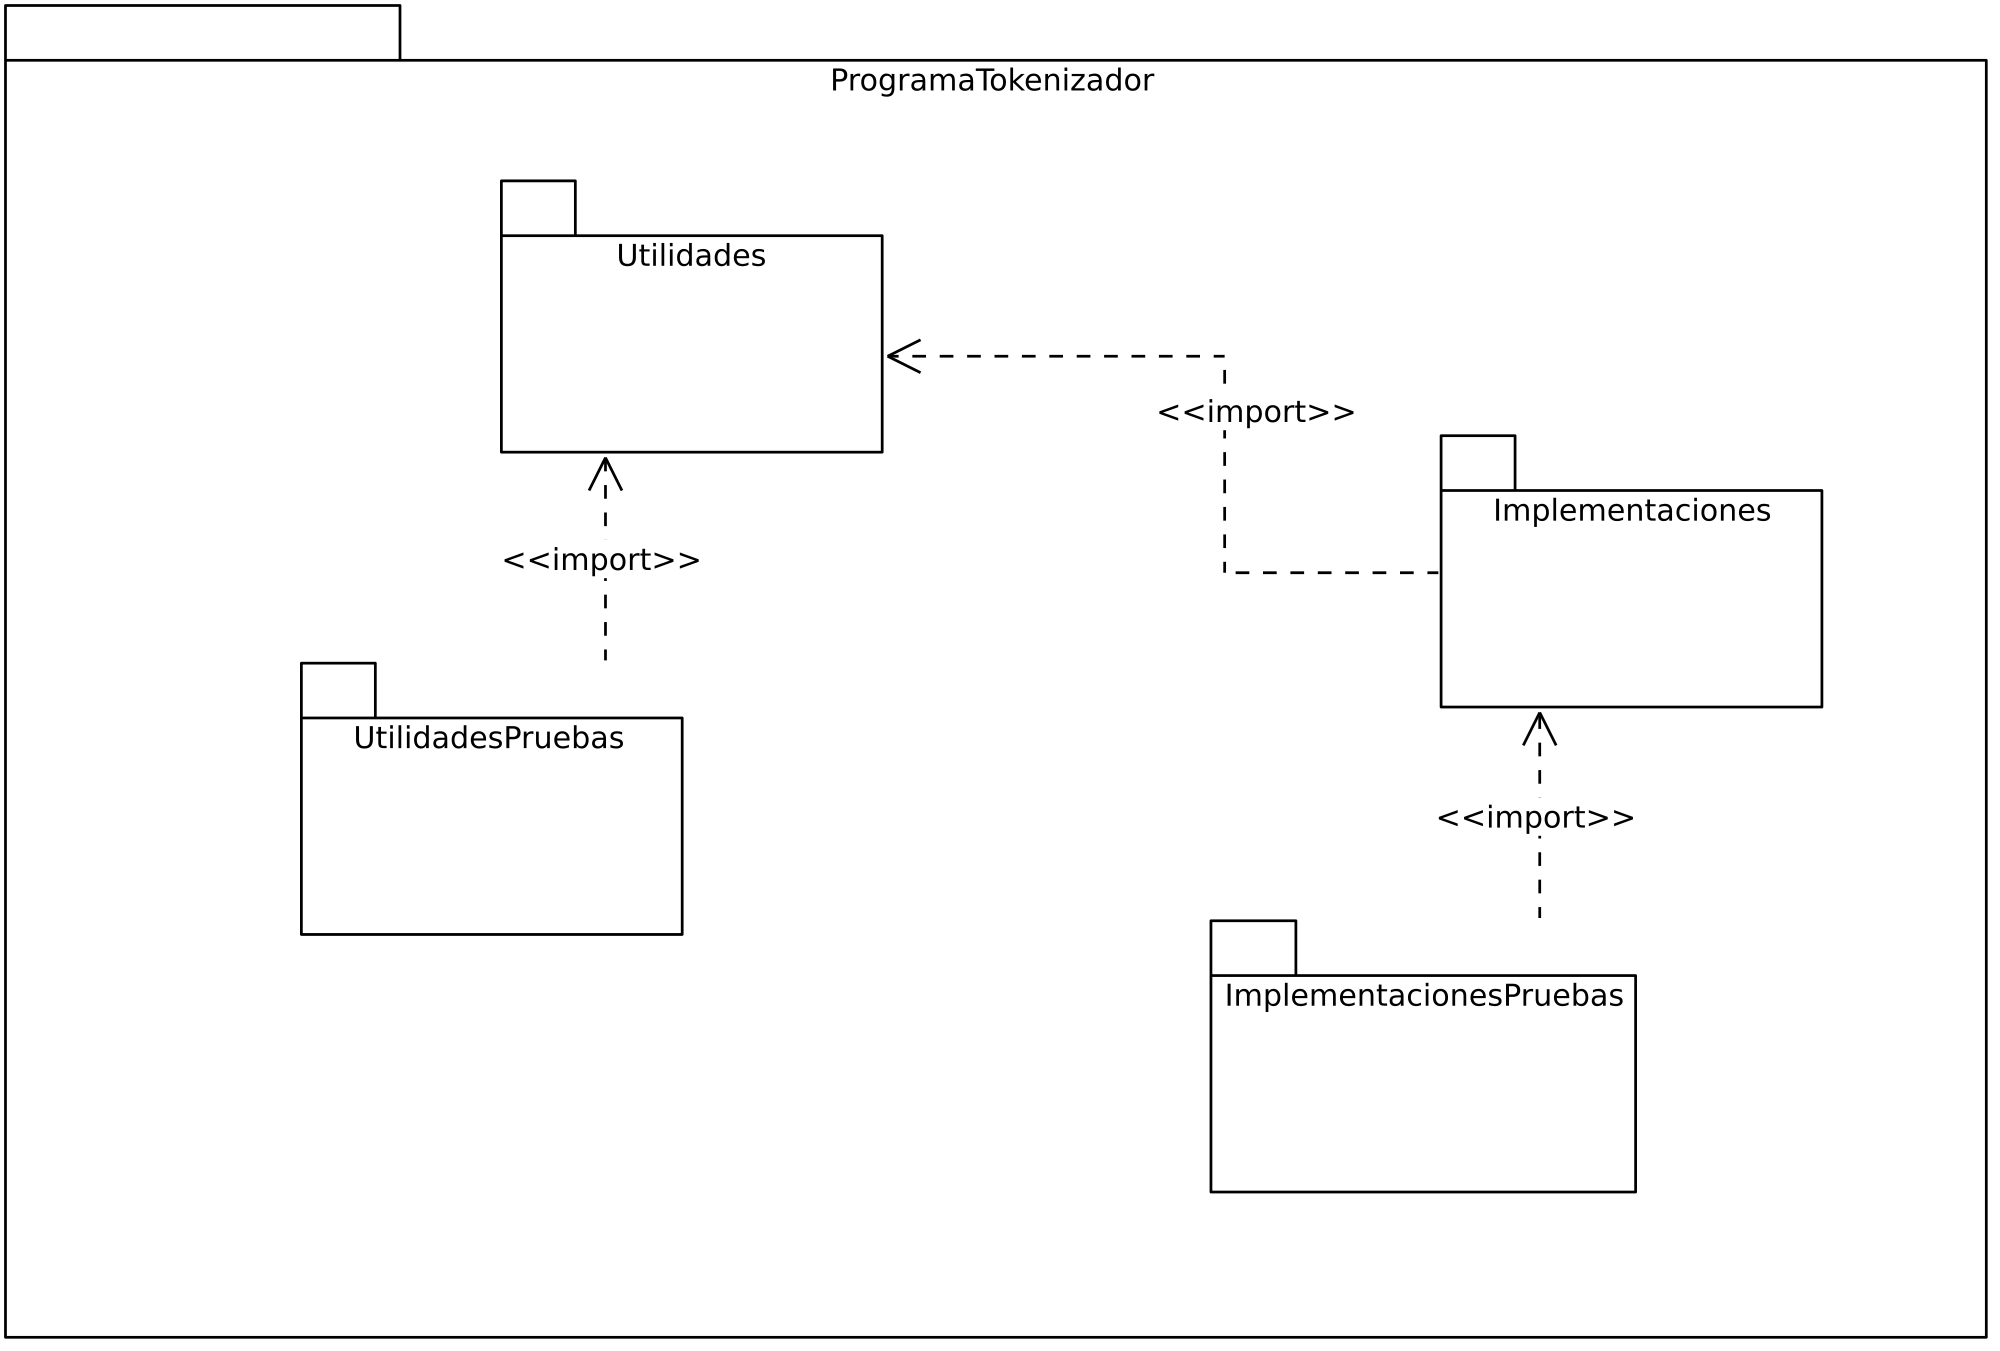
\includegraphics[width=0.6\linewidth]{diagramas/paquetes.png}
    \caption{Diagrama de dependencias entre paquetes.}
    \label{paquetes_general}
  \end{center}
\end{figure}

\subimport{/}{ffx}
\subimport{/}{bps}
\subimport{/}{tkr}
\subimport{/}{ahr}
\subimport{/}{drbg}
\subimport{/}{pruebas}
